%% AMS-LaTeX Created with the Wolfram Language : www.wolfram.com

\documentclass{article}
\usepackage{amsmath, amssymb, graphics, setspace}

\newcommand{\mathsym}[1]{{}}
\newcommand{\unicode}[1]{{}}

\newcounter{mathematicapage}
\begin{document}

\begin{doublespace}
\noindent\(\pmb{\text{$\$$Assumptions} \text{Element}[x, \text{PositiveIntegers}]}\\
\pmb{\text{$\$$Assumptions} \text{Element}[t, \text{PositiveIntegers}]}\\
\pmb{\text{$\$$Assumptions} \text{Element}[N, \text{PositiveIntegers}]}\\
\pmb{}\\
\pmb{P[\text{i$\_$},\text{t$\_$}] \text{:=} 1/N +\text{  }2/N *\text{Sum}[}\\
\pmb{\text{Cos}[(i-1/2)*\text{   }\text{Pi} * k / N ] * \text{Cos}[\text{  }\text{Pi} * k / N/2 ] {}^{\wedge} (2*t +1),}\\
\pmb{\{k, 1, N-1\}}\\
\pmb{]\text{  }}\)
\end{doublespace}

\begin{doublespace}
\noindent\(\text{True} (x\in \mathbb{Z}\&\&x>0)\)
\end{doublespace}

\begin{doublespace}
\noindent\(\text{True} (t\in \mathbb{Z}\&\&t>0)\)
\end{doublespace}

\begin{doublespace}
\noindent\(\text{True} (N\in \mathbb{Z}\&\&N>0)\)
\end{doublespace}

Now we consider the difference of P(t) and P(t + 1) . We want to see the converge rate of P .\\
\\
The difference of P { }= \(\(\frac{2 \sum _{k=1}^{-1+N} \text{Cos}\left[\frac{k \pi }{2 N}\right]^{1+2 t} \text{Cos}\left[\frac{k \pi  \left(-\frac{1}{2}+x\right)}{N}\right]}{N}-\frac{2
\sum _{k=1}^{-1+N} \text{Cos}\left[\frac{k \pi }{2 N}\right]^{1+2 (1+t)} \text{Cos}\left[\frac{k \pi  \left(-\frac{1}{2}+x\right)}{N}\right]}{N}\)\)
{ } ,\\
while the middle term \(\(\sum _{k=1}^{-1+N} \text{Cos}\left[\frac{k \pi }{2 N}\right]^{1+2 t} \text{Cos}\left[\frac{k \pi  \left(-\frac{1}{2}+x\right)}{N}\right]-\text{Cos}\left[\frac{k
\pi }{2 N}\right]^{1+2 (1+t)} \text{Cos}\left[\frac{k \pi  \left(-\frac{1}{2}+x\right)}{N}\right]\)\) could be simplified.

\begin{doublespace}
\noindent\(\pmb{\text{Cos}\left[\frac{k \pi }{2 N}\right]^{1+2 t} \text{Cos}\left[\frac{k \pi  \left(-\frac{1}{2}+x\right)}{N}\right]-\text{Cos}\left[\frac{k
\pi }{2 N}\right]^{1+2 (1+t)} \text{Cos}\left[\frac{k \pi  \left(-\frac{1}{2}+x\right)}{N}\right] \text{//} \text{Simplify}}\)
\end{doublespace}

\begin{doublespace}
\noindent\(\text{Cos}\left[\frac{k \pi }{2 N}\right]^{1+2 t} \text{Cos}\left[\frac{k \pi  \left(-\frac{1}{2}+x\right)}{N}\right] \text{Sin}\left[\frac{k
\pi }{2 N}\right]^2\)
\end{doublespace}

Thus, we consider the Pdiff as 

\begin{doublespace}
\noindent\(\pmb{\text{Pdiff}[\text{x$\_$}, \text{t$\_$}] \text{:=} \frac{2}{N} \sum _{k=1}^{-1+N} \text{   }\text{Cos}\left[\frac{k \pi }{2 N}\right]^{1+2
t} \text{Cos}\left[\frac{k \pi  \left(-\frac{1}{2}+x\right)}{N}\right] \text{Sin}\left[\frac{k \pi }{2 N}\right]^2}\\
\pmb{\text{termInPdiff}[\text{k$\_$}, \text{x$\_$}, \text{t$\_$}] \text{:=} \text{Cos}\left[\frac{k \pi }{2 N}\right]^{1+2 t} \text{Cos}\left[\frac{k
\pi  \left(-\frac{1}{2}+x\right)}{N}\right] \text{Sin}\left[\frac{k \pi }{2 N}\right]^2}\)
\end{doublespace}

\(\(\left(\sum _{k=1}^{-1+N} \text{   }\text{Cos}\left[\frac{k \pi }{2 N}\right]^{1+2 t} \text{Cos}\left[\frac{k \pi  \left(-\frac{1}{2}+x\right)}{N}\right]
\text{Sin}\left[\frac{k \pi }{2 N}\right]^2 \right){}^2\text{  }\text{$<$=} \unicode{ff08} \sum _{k=1}^{-1+N} \text{Cos}\left[\frac{k \pi }{2 N}\right]^{2+4t}
\unicode{ff09}\unicode{ff08}\sum _{k=1}^{-1+N}  \text{Cos}\left[\frac{k \pi  \left(-\frac{1}{2}+x\right)}{N}\right]^2 \text{Sin}\left[\frac{k \pi
}{2 N}\right]^4\unicode{ff09}\text{   }\)\) \\
Thus, we want to bond the l.h.s by the r.h.s.\\


\begin{doublespace}
\noindent\(\pmb{\sum _{k=1}^{-1+N} \text{Cos}\left[\frac{k \pi }{2 N}\right]^{2+4t}}\\
\pmb{\sum _{k=1}^{-1+N}  \text{Cos}\left[\frac{k \pi  \left(-\frac{1}{2}+x\right)}{N}\right]^2 \text{Sin}\left[\frac{k \pi }{2 N}\right]^4}\)
\end{doublespace}

\begin{doublespace}
\noindent\(\sum _{k=1}^{-1+N} \text{Cos}\left[\frac{k \pi }{2 N}\right]^{2+4 t}\)
\end{doublespace}

\begin{doublespace}
\noindent\(\pmb{\text{{``} The result of the second term is{''}}}\\
\pmb{\text{sdTerm}[\text{x$\_$}] \text{:=} \frac{1}{64} \left(-12+12 N+8 \text{Cos}\left[\frac{(-1+N) \pi }{2 N}\right] \text{Csc}\left[\frac{\pi
}{2 N}\right]+8 \text{Cos}\left[\frac{(1+N) \pi }{2 N}\right] \text{Csc}\left[\frac{\pi }{2 N}\right]-2 \text{Cos}\left[\frac{(-2+N) \pi }{2 N}\right]
\text{Csc}\left[\frac{\pi }{N}\right]+2 \text{Cos}\left[\frac{(2+N) \pi }{2 N}\right] \text{Csc}\left[\frac{\pi }{N}\right]+4 \text{Cos}\left[\frac{-N
\pi +2 \pi  x}{2 N}\right] \text{Csc}\left[\frac{\pi  x}{N}\right]-4 \text{Cos}\left[\frac{-N \pi -2 \pi  x+4 N \pi  x}{2 N}\right] \text{Csc}\left[\frac{\pi
 x}{N}\right]\right)}\\
\pmb{\text{sdTerm}[1/2]}\)
\end{doublespace}

\begin{doublespace}
\noindent\(\text{ The result of the second term is}\)
\end{doublespace}

\begin{doublespace}
\noindent\(\frac{1}{64} \left(-12+12 N+8 \text{Cos}\left[\frac{(-1+N) \pi }{2 N}\right] \text{Csc}\left[\frac{\pi }{2 N}\right]+8 \text{Cos}\left[\frac{(1+N)
\pi }{2 N}\right] \text{Csc}\left[\frac{\pi }{2 N}\right]+4 \text{Cos}\left[\frac{\pi -N \pi }{2 N}\right] \text{Csc}\left[\frac{\pi }{2 N}\right]-4
\text{Cos}\left[\frac{-\pi +N \pi }{2 N}\right] \text{Csc}\left[\frac{\pi }{2 N}\right]-2 \text{Cos}\left[\frac{(-2+N) \pi }{2 N}\right] \text{Csc}\left[\frac{\pi
}{N}\right]+2 \text{Cos}\left[\frac{(2+N) \pi }{2 N}\right] \text{Csc}\left[\frac{\pi }{N}\right]\right)\)
\end{doublespace}

We want the upper bond of the second term. And we know \(0<\) when \(\), { }Thus, the upper term is less than\\


\begin{doublespace}
\noindent\(\pmb{\text{}}\\
\pmb{D[\text{sdTerm}[x], x] *64N \text{//} \text{Simplify}}\)
\end{doublespace}

\begin{doublespace}
\noindent\(4 \pi  \text{Csc}\left[\frac{\pi  x}{N}\right]^2 \left(-((-1+N) \text{Sin}[2 \pi  x])+N \text{Sin}\left[\frac{2 (-1+N) \pi  x}{N}\right]\right)\)
\end{doublespace}

\begin{doublespace}
\noindent\(\pmb{f[\text{x$\_$}]\text{:=}(N-1) \text{Sin}[2 \pi  x]+N \text{Sin}\left[\frac{2 (-1+N) \pi  x}{N}\right] }\\
\pmb{f[N/2]}\)
\end{doublespace}

\begin{doublespace}
\noindent\(N \text{Sin}[(-1+N) \pi ]+(-1+N) \text{Sin}[N \pi ]\)
\end{doublespace}

\begin{doublespace}
\noindent\(\pmb{\text{sdTerm}[N/2]}\)
\end{doublespace}

\begin{doublespace}
\noindent\(\frac{1}{64} \left(-8+12 N-4 \text{Cos}\left[\frac{-2 N \pi +2 N^2 \pi }{2 N}\right]+8 \text{Cos}\left[\frac{(-1+N) \pi }{2 N}\right]
\text{Csc}\left[\frac{\pi }{2 N}\right]+8 \text{Cos}\left[\frac{(1+N) \pi }{2 N}\right] \text{Csc}\left[\frac{\pi }{2 N}\right]-2 \text{Cos}\left[\frac{(-2+N)
\pi }{2 N}\right] \text{Csc}\left[\frac{\pi }{N}\right]+2 \text{Cos}\left[\frac{(2+N) \pi }{2 N}\right] \text{Csc}\left[\frac{\pi }{N}\right]\right)\)
\end{doublespace}

\begin{doublespace}
\noindent\(\pmb{\frac{1}{64} \left(-8+12 N-4 \text{Cos}\left[\frac{-2 N \pi +2 N^2 \pi }{2 N}\right]+8 \text{Cos}\left[\frac{(-1+N) \pi }{2 N}\right]
\text{Csc}\left[\frac{\pi }{2 N}\right]+8 \text{Cos}\left[\frac{(1+N) \pi }{2 N}\right] \text{Csc}\left[\frac{\pi }{2 N}\right]-2 \text{Cos}\left[\frac{(-2+N)
\pi }{2 N}\right] \text{Csc}\left[\frac{\pi }{N}\right]+2 \text{Cos}\left[\frac{(2+N) \pi }{2 N}\right] \text{Csc}\left[\frac{\pi }{N}\right]\right)
\text{//} \text{Simplify}}\)
\end{doublespace}

\begin{doublespace}
\noindent\(\pmb{\frac{1}{16} (-3+3 N+\text{Cos}[N \pi ])}\)
\end{doublespace}

So the second term is less than \(\frac{1}{16}(-2+3N)\)\\
When it comes to the first term, we make the following approximation:\\
\(\sum _{k=1}^{-1+N} \text{Cos}\left[\frac{k \pi }{2 N}\right]^{2+4t} \text{-$>$}\text{  }\frac{N}{\pi }\sum _{k=1}^{-1+N} \frac{\pi }{N}\text{Cos}\left[\frac{k
\pi }{2 N}\right]^{2+4t} \text{-$>$} \frac{N}{\pi }\int \text{d$\kappa $} \text{Cos}\left[\frac{\kappa }{2 }\right]^{2+4t}\) 

\begin{doublespace}
\noindent\(\pmb{\int_0^{\pi } \text{Cos}\left[\frac{\kappa }{2 }\right]^{2+4t} \, d\kappa }\)
\end{doublespace}

\begin{doublespace}
\noindent\(\fbox{$\frac{\sqrt{\pi } \text{Gamma}\left[\frac{3}{2}+2 t\right]}{\text{Gamma}[2+2 t]}\text{ if }\text{Re}[t]>-\frac{3}{4}$}\)
\end{doublespace}

Thus, the term \(\sum _{k=1}^{-1+N} \text{Cos}\left[\frac{k \pi }{2 N}\right]^{2+4t}\) could be approximated by \(\(\frac{N}{\surd \pi }\frac{ \text{Gamma}\left[\frac{3}{2}+2
t\right]}{\text{Gamma}[2+2 t]}\)\)

\begin{doublespace}
\noindent\(\pmb{\text{Plot}\left[\left\{\sum _{k=1}^{-1+200} \text{Cos}\left[\frac{k \pi }{2 *200}\right]^{2+4t}, \frac{200}{\text{Pi}}*\frac{\sqrt{\pi
} \text{Gamma}\left[\frac{3}{2}+2 t\right]}{\text{Gamma}[2+2 t]}\right\}, \{t,10,1000\}, \text{PlotLabels}\to \text{{``}Expressions{''}}\right]}\)
\end{doublespace}

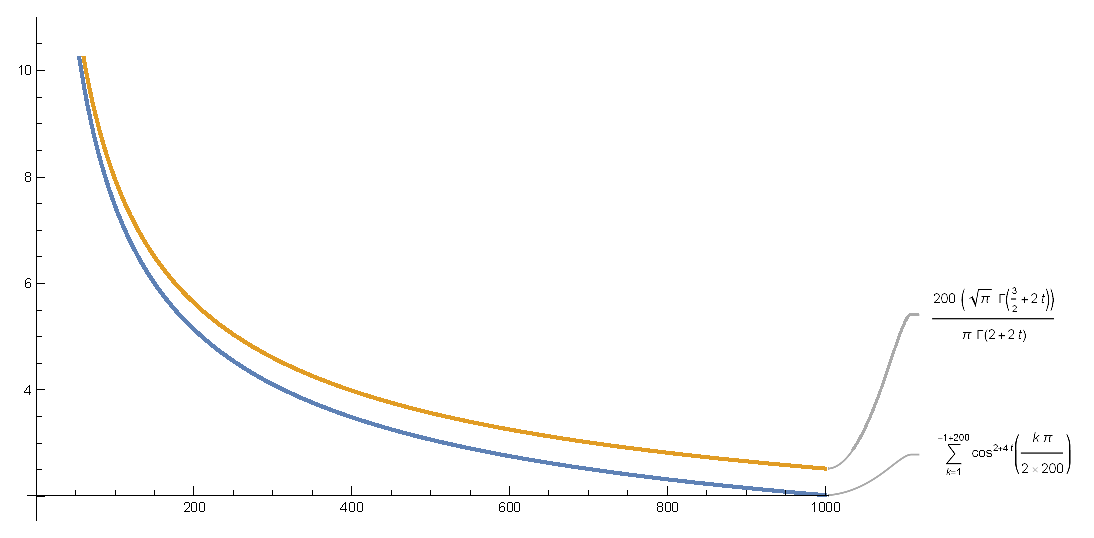
\includegraphics{DealingP_gr1.eps}

\begin{doublespace}
\noindent\(\pmb{\text{}}\)
\end{doublespace}

\begin{doublespace}
\noindent\(\pmb{\fbox{$\text{Series}$}\left[\frac{\text{Gamma}\left[\frac{3}{2}+\frac{2}{w}\right]}{\text{Gamma}\left[2+\frac{2 }{w}\right]},\{w,0,2\}\right]}\)
\end{doublespace}

\begin{doublespace}
\noindent\(\text{RefLink}\left[\text{Series},\text{paclet}:\frac{\text{ref}}{\text{Series}}\right]\left[\frac{\text{Gamma}\left[\frac{3}{2}+\frac{2}{w}\right]}{\text{Gamma}\left[2+\frac{2}{w}\right]},\{w,0,2\}\right]\)
\end{doublespace}

\begin{doublespace}
\noindent\(\pmb{\text{Series}\left[\frac{\text{Gamma}\left[\frac{3}{2}+\frac{2}{w}\right]}{\text{Gamma}\left[2+\frac{2}{w}\right]},\{w,0,2\}, \text{Assumptions}\text{-$>$}w>0\right]}\)
\end{doublespace}

\begin{doublespace}
\noindent\(\frac{\sqrt{w}}{\sqrt{2}}-\frac{5 w^{3/2}}{16 \sqrt{2}}+O[w]^{5/2}\)
\end{doublespace}

\begin{doublespace}
\noindent\(\pmb{\text{Series}[\text{Gamma}[x],\{x,0,2\}]}\)
\end{doublespace}

\begin{doublespace}
\noindent\(\frac{1}{x}-\text{EulerGamma}+\frac{1}{12} \left(6 \text{EulerGamma}^2+\pi ^2\right) x+\frac{1}{6} \left(-\text{EulerGamma}^3-\frac{\text{EulerGamma}
\pi ^2}{2}+\text{PolyGamma}[2,1]\right) x^2+O[x]^3\)
\end{doublespace}

\end{document}
